\documentclass{article}

\usepackage{amsmath,amssymb}
\usepackage{tikz}
\usepackage{pgfplots}
\usepackage{xcolor}
\usepackage[left=2.1cm,right=3.1cm,bottom=3cm,footskip=0.75cm,headsep=0.5cm]{geometry}
\usepackage{enumerate}
\usepackage{enumitem}
\usepackage{marvosym}
\usepackage{tabularx}
\usepackage{multirow}
\usepackage[colorlinks = true, linkcolor = blue, urlcolor  = blue, citecolor = blue, anchorcolor = blue]{hyperref}
\usepackage{ulem}

\usepackage{listings}
\definecolor{lightlightgray}{rgb}{0.95,0.95,0.95}
\definecolor{lila}{rgb}{0.8,0,0.8}
\definecolor{mygray}{rgb}{0.5,0.5,0.5}
\definecolor{mygreen}{rgb}{0,0.8,0.26}
\lstdefinestyle{html} {language=html}
\lstset{language=html,
	basicstyle=\ttfamily,
	keywordstyle=\color{lila},
	commentstyle=\color{lightgray},
	stringstyle=\color{mygreen}\ttfamily,
	backgroundcolor=\color{white},
	showstringspaces=false,
	numbers=left,
	numbersep=10pt,
	numberstyle=\color{mygray}\ttfamily,
	identifierstyle=\color{blue},
	xleftmargin=.1\textwidth, 
	%xrightmargin=.1\textwidth,
	escapechar=§,
	breaklines=true,
	postbreak=\mbox{\space}
}
\lstset{literate=%
	{Ö}{{\"O}}1
	{Ä}{{\"A}}1
	{Ü}{{\"U}}1
	{ß}{{\ss}}1
	{ü}{{\"u}}1
	{ä}{{\"a}}1
	{ö}{{\"o}}1
}

\usepackage[utf8]{inputenc}

\renewcommand*{\arraystretch}{1.4}

\newcolumntype{L}[1]{>{\raggedright\arraybackslash}p{#1}}
\newcolumntype{R}[1]{>{\raggedleft\arraybackslash}p{#1}}
\newcolumntype{C}[1]{>{\centering\let\newline\\\arraybackslash\hspace{0pt}}m{#1}}

\newcommand{\E}{\mathbb{E}}
\DeclareMathOperator{\rk}{rk}
\DeclareMathOperator{\Var}{Var}
\DeclareMathOperator{\Cov}{Cov}
\DeclareMathOperator{\SD}{SD}
\DeclareMathOperator{\Cor}{Cor}

\title{\textbf{Barrierefreie Dokumente, Übung 1}}
\author{\textsc{Henry Haustein}, \textsc{Dennis Rössel}}
\date{}

\begin{document}
	\maketitle
	
	\section*{Aufgabe 0: Vorbereitung zum Übungsprojekt}
	Wir nehmen die Webseite der Stadt Dresden, \url{www.dresden.de}.
	
	\section*{Aufgabe 1.1: Das Web ohne Maus erkunden}
	\begin{enumerate}[label=(\alph*)]
		\item Unsere 2 Tasks sind:
		\begin{itemize}
			\item Erreichen der Unterseite zur Barrierefreiheit
			\item Informationen zur Beantragung eines Personalausweises
		\end{itemize}
		\item Dokumentation
		\begin{itemize}
			\item Zweites mal TAB drücken führt in die Suchleiste, dort dann Eingabe von \textit{Barrierefreiheit} und ENTER drücken. Zweites Suchergebnis enthält die gewünschte Seite. Problematisch bei der Suchergebnis-Seite ist, dass man zuerst durch das gesamte Menü muss, bevor man zu den Suchergebnissen mittels TAB kommt.
			\item Ähnlich wie zum ersten Task wurde die Suchfunktion benutzt. Der erste Treffer führt direkt zur passenden Seite, aber auch hier muss man erst durch das gesamte Menü navigieren, bis man zum Inhalt kommt. Aufklappen der Textelemente funktioniert gut.
		\end{itemize}
	\end{enumerate}

	\section*{Aufgabe 1.2: One-Pager mit ARIA annotieren}
	\begin{enumerate}[label=(\alph*)]
		\item Webseite zur Erklärung der Barrierefreiheit stark eingekürzt und mit ARIA-Tags versehen:
		\begin{lstlisting}[style=html,tabsize=2]
<!DOCTYPE html>
<html lang="de">
	<head>
		<meta charset="UTF-8">
		<meta http-equiv="X-UA-Compatible" content="IE=edge">
		<meta name="viewport" content="width=device-width, initial-scale=1.0">
		<title>Document</title>
	</head>
	<body>
		<div id="inhalt">
			<ul>
				<li class="listitem" aria-label="Navigation zur Startseite"><a href="index.html">Dresden</a></li>
				<li class="listitem" aria-label="Navigation zu Rathaus Seite"><a href="Rathaus.html">Rathaus</a></li>
				<li class="listitem" aria-label="Navigation zu Leben in Dresden"><a href="Leben_in_Dresden.html">Leben in Dresden</a></li>
				<li class="listitem" aria-label="Navigation zu Stadtraum"><a href="Stadtraum.html">Stadtraum</a></li>
				<li class="listitem" aria-label="Navigation zu Wirtschaft"><a href="Wirtschaft.html">Wirtschaft</a></li>
				<li class="listitem" aria-label="Navigation zu Kultur"><a href="Kultur.html">Kultur</a></li>
				<li class="listitem" aria-label="Navigation zu Tourismus"><a href="Tourismus.html">Tourismus</a></li>
			</ul>
		</div>
		<main>
			<div>
				<h1>Menschen mit Behinderung</h1>
			</div>
			<div class="text">
				<table id="tabelle">
					<tr>
						<td><a href="" aria-label="">Beauftragte für Menschen mit Behinderung</a></td>
						<td><a href="" aria-label="">Aktionsplan zur Umsetzung der UN-BRK</a></td>
						<td><a href="" aria-label="">Aktuelles</a></td>
						<td><a href="" aria-label="">Bildung & Arbeit</a></td>
					</tr>
					<tr>
						<td><a href="" aria-label="">Mobilität & Wohnen</a></td>
						<td><a href="" aria-label="">Infoportal Barrierefreiheit</a></td>
						<td><a href="" aria-label="">Kultur - Freizeit - Sport</a></td>
						<td><a href="" aria-label="">Gesundheit & Pflege</a></td>
					</tr>
					<tr>
						<td><a href="" aria-label="">Barrierefreie Kommunikatio</a>n</td>
						<td><a href="" aria-label="">Information & Beratung</a></td>
					</tr>
				</table>
			</div>
			<div>
				<h2>Menschen mit Behinderungen in der Landeshauptstadt Dresden</h2>
			</div>
			<div role="main">
				Etwa jeder zehnte Bürger der Landeshauptstadt Dresden lebt mit einer Behinderung. 
				Für diese Menschen ist es wichtig, dass sie ihren Alltag weitgehend selbstständig und selbstbestimmt meistern können. 
				Dazu bedarf es der barrierefreien Stadt.
			</div>
			<br>
			<a href="www.facebook.com/Dresden">
				<button>
					<span aria-label="Facebook Link">
						<strong>F</strong>
					</span>  
				</button>
			</a>
		</main>
	</body>
</html>
		\end{lstlisting}
		\item Auswertung mittels WAVE-Tool
		\begin{center}
			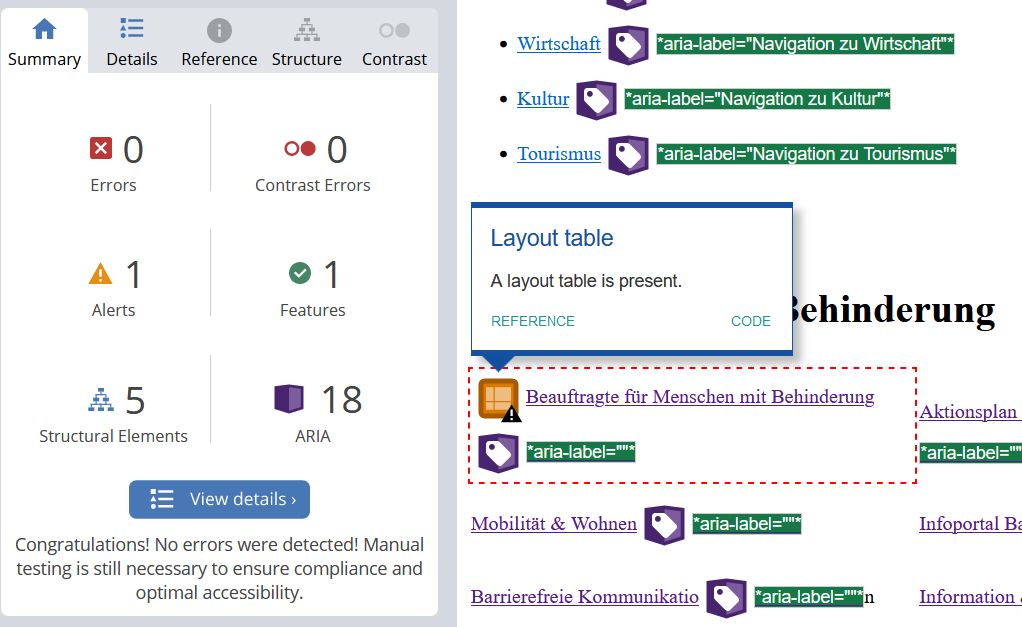
\includegraphics[scale=0.4]{image001.png}
		\end{center}
		\item Es wird die Layout-Tabelle angekreidet, aber diese wurde mittels \texttt{aria-label=""} entschärft für den Screen-Reader. Laut dem WAVE-Tool ist die Seite sehr gut barrierefrei, aber das Tool überprüft nicht, ob die Labels, die gesetzt wurden, auch richtig in dem Kontext sind.
	\end{enumerate}
	
	\section*{Aufgabe 1.3: Website nach WCAG begutachten}
	\begin{enumerate}[label=(\alph*)]
		\item Untersuchung von \url{www.dresden.de} mit Ziel-Konformitätsstufe AA.
		\item Folgende Seiten werden untersucht:
		\begin{itemize}
			\item Startseite: \url{https://www.dresden.de/index_de.php}
			\item Erklärung zur Barrierefreiheit: \url{https://www.dresden.de/de/sonstiges/erklaerung-zur-barrierefreiheit.php}
			\item Suchergebnisseite mit Keyword \textit{Barrierefreiheit}: \url{https://www.dresden.de/suche/?q=Barrierefreiheit&q1=&lang=de}
		\end{itemize}
		\item Prüfbericht zur Startseite
		\begin{center}
			\begin{tabular}{l|c|L{7cm}}
				\textbf{Prüfschritt} & \textbf{Level} & \textbf{Bemerkungen} \\
				\hline
				Missing alternative Text & A & \multirow{2}{7cm}{Element ist auf Desktop-Seite nicht zu sehen, bei Blick in den Quelltext offenbart sich, dass es sich um Werbung handelt.} \\
				Empty Links & A & \\
				keine H1 Überschrift & A, AA & \\
				zu wenig Kontrast & A & betrifft Bild auf Startseite und zugehörigen Text \textit{Coronavirus: Impfung, Maßnahmen, Hilfe für Betroffene} und \textit{Mehr Informationen} \\
				Layout-Tabelle & A & Beim Drucken werden grundsätzliche Informationen wie Seite und Datum/Uhrzeit mit auf den Ausdruck gesetzt, diese sind aber auf der Desktop-Seite unsichtbar. Aber ein Screenreader würde den Text vorlesen, weil die passenden ARIA-Labels fehlen.
			\end{tabular}
		\end{center}
		\item Prüfbericht zur Erklärung zur Barrierefreiheit
		\begin{center}
			\begin{tabular}{l|c|L{7cm}}
				\textbf{Prüfschritt} & \textbf{Level} & \textbf{Bemerkungen} \\
				\hline
				Missing alternative Text & A & \multirow{2}{7cm}{Element ist auf Desktop-Seite nicht zu sehen, bei Blick in den Quelltext offenbart sich, dass es sich um Werbung handelt.} \\
				Empty Links & A & \\
				keine H2 Überschrift & A, AA & Es gibt eine H1 und eine H3 Überschrift, aber keine H2 Überschrift\\
				zu wenig Kontrast & A & betrifft alle Links auf der Webseite, die in dem Ocker-Ton geschrieben sind \\
				Layout-Tabelle & A & Beim Drucken werden grundsätzliche Informationen wie Seite und Datum/Uhrzeit mit auf den Ausdruck gesetzt, diese sind aber auf der Desktop-Seite unsichtbar. Aber ein Screenreader würde den Text vorlesen, weil die passenden ARIA-Labels fehlen.
			\end{tabular}
		\end{center}
		\item Prüfbericht zur Suche
		\begin{center}
			\begin{tabular}{l|c|L{7cm}}
				\textbf{Prüfschritt} & \textbf{Level} & \textbf{Bemerkungen} \\
				\hline
				Missing alternative Text & A & \multirow{2}{7cm}{Element ist auf Desktop-Seite nicht zu sehen, bei Blick in den Quelltext offenbart sich, dass es sich um Werbung handelt.} \\
				Empty Links & A & \\
				kein Label & A, AA & Suchleiste hat kein \texttt{label}-Attribut, Filter hat ein leeres bzw. fehlendes \texttt{label}-Attribut \\
				Sprachangabe fehlt & A & \\
				kein Alternativtext im Link & A & weiter-Button für die nächste Suchergebnisseite hat keinen Alternativtext \\
				keine H1 Überschrift & A, AA & \\
				Javascript Jump Menu & A & Filter enthalten Javascript, was bei einem onchange-Event ausgelöst wird \\
				zu wenig Kontrast & A & betrifft alle Links auf der Webseite, die in dem Ocker-Ton geschrieben sind \\
				Layout-Tabelle & A & Beim Drucken werden grundsätzliche Informationen wie Seite und Datum/Uhrzeit mit auf den Ausdruck gesetzt, diese sind aber auf der Desktop-Seite unsichtbar. Aber ein Screenreader würde den Text vorlesen, weil die passenden ARIA-Labels fehlen.
			\end{tabular}
		\end{center}
	\end{enumerate}
	
\end{document}